%
% 6.006 problem set 3 solutions template
%
\documentclass[12pt,twoside]{article}

\usepackage{amsmath}
\usepackage{color}
\usepackage{tikz}

\input{macros}

\setlength{\oddsidemargin}{0pt}
\setlength{\evensidemargin}{0pt}
\setlength{\textwidth}{6.5in}
\setlength{\topmargin}{0in}
\setlength{\textheight}{8.5in}

\newcommand{\theproblemsetnum}{3}
\newcommand{\releasedate}{Thursday, October 20, 2016}
\newcommand{\partaduedate}{Tuesday, November 1, 2016}
\newcommand{\tabUnit}{3ex}
\newcommand{\tabT}{\hspace*{\tabUnit}}

\title{6.006 Problem Set 3}

\begin{document}

\handout{Problem Set \theproblemsetnum}{Thursday, October 20, 2016}

\textbf{All parts are due {\bf \partaduedate} at {\bf 11:59PM}}.

\setlength{\parindent}{0pt}

\medskip

\hrulefill

\medskip

{\bf Name:} Dimitris Koutentakis

\medskip

{\bf Collaborators:} Nestoras Hahamis, Carl Unger 

\medskip

\hrulefill

%%%%%%%%%%%%%%%%%%%%%%%%%%%%%%%%%%%%%%%%%%%%%%%%%%%%%
% See below for common and useful latex constructs. %
%%%%%%%%%%%%%%%%%%%%%%%%%%%%%%%%%%%%%%%%%%%%%%%%%%%%%

% Some useful commands:
%$f(x) = \Theta(x)$
%$T(x, y) \leq \log(x) + 2^y + \binom{2n}{n}$
% {\tt code\_function}


% You can create unnumbered lists as follows:
%\begin{itemize}
%    \item First item in a list 
%        \begin{itemize}
%            \item First item in a list 
%                \begin{itemize}
%                    \item First item in a list 
%                    \item Second item in a list 
%                \end{itemize}
%            \item Second item in a list 
%        \end{itemize}
%    \item Second item in a list 
%\end{itemize}

% You can create numbered lists as follows:
%\begin{enumerate}
%    \item First item in a list 
%    \item Second item in a list 
%    \item Third item in a list
%\end{enumerate}

% You can write aligned equations as follows:
%\begin{align} 
%    \begin{split}
%        (x+y)^3 &= (x+y)^2(x+y) \\
%                &= (x^2+2xy+y^2)(x+y) \\
%                &= (x^3+2x^2y+xy^2) + (x^2y+2xy^2+y^3) \\
%                &= x^3+3x^2y+3xy^2+y^3
%    \end{split}                                 
%\end{align}

% You can create grids/matrices as follows:
%\begin{align}
%    A = 
%    \begin{bmatrix}
%        A_{11} & A_{21} \\
%        A_{21} & A_{22}
%    \end{bmatrix}
%\end{align}

\begin{problems}

\section*{Part A}

\problem  % Problem 1

\begin{problemparts}
\problempart 

The Algorithm of choice for sorting the buildings by number, would be radix sort. In specific, we would sort the buildings d times, once for every digit. We would start by the last digit and sort the numbers based on that digit using a stable sort algorithm (e.g. counting sort). Next, we would perform the same stable sorting on the digit to the left. We will repeat this until we reach the left-most digit of the number d.
\\
\\
This will result in a sorted list of all the buildings. Since we have to sort O(d) digits and every sort needs to do O(n) comparisons, the total time for sorting the buildings would be $T(n)=O(dn)$.

\problempart 
In order to find the order of traversal of buildings along the $i$-artery, we will need to basically sort the buildings according to their $i^{ith}$ digit. Since the buildings are already sorted, we can use a version of binary search in order to achieve that.
\\\\
In specific, we can start by doing a binary search for the first building in that artery. Namely we search for the building in the I-artery with the $i^{ith}$ digit to be 0 and repeat for all 10 buildings in the artery. 
Since we have n numbers that can be organized in a Binary Search tree of height $h=logn$, we need to do $O(logn)$ comparisons. Also each comparison takes $O(d)$ time, since we have d digits. Since this will be performed at most 10 times, the runtime of this algorithm would be $T(n)=O(d logn)$.
 

\end{problemparts}

\problem  % Problem 2

\begin{problemparts}
\problempart
In order to find the kth largest element in these two arrays, we can perform a version of parallel binary search, according to the following algorithm.
\\\\
Assume we have the two arrays A1 and A2.  Let's begin by searching array A1 to see if it has the kth largest value. We know for a fact that the kth largest value can't appear in the array in array A1 after position k (assuming all the elements are distinct). So let's focus just on the the first k elements of array A1. We'll do a binary search over these values as follows. Start at position k/2; this is the k/2th largest element in array A1. Now do a binary search in array A2 to find the largest value in A2 smaller than this value and look at its position in the array; this is the number of elements in A2 smaller than the current value. If we add up the position of the elements in A1 and A2, we have the total number of elements in the two arrays smaller than the current element. If this is exactly k, we're done. If this is less than k, then we recurse in the upper half of the first k elements of A1, and if this is greater than k we recurse in the lower half of the first elements of k, etc. Eventually, we'll either find that the kth largest element is in array A1, in which case we're done. Otherwise, repeat this process on array A2.
\\\\
The runtime for this algorithm is as follows. The search of array A1 does a binary search over k elements, which takes O(lg k) iterations. Each iteration costs O(lg n), since we have to do a binary search in A2. This means that the total time for this search is O(lg k lg n). The time to do this in array A2 is the same, so the net runtime for the algorithm is $O(lg k lg n) = O(lg^2 n)$.
\problempart 
We can modify the regular AVL-insert to keep track of the size of the subtree rooted at x, by changing both the insertion of a node and the rotations. In the first part, we need to increment the size attribute of each node on the path from the root to the end of the tree by one. Secondly, in each rotation, we need to do the following. For example in a left rotation, we need to first change the right right child's size to the parent's size and then update the root's size to be the sum of it's new left child's size plus it's right child's size plus 1. This will take O(lgn) time, since there are O(lgn) nodes on the path traversed and we only need to take care of O(1) nodes in each rotation.

\problempart
Since we have the size attribute for each node, the answer is very similar to (a).
\\\\
Assume we have the two AVL trees with size pointers at the nodes T1 and T2.  Let's begin by searching tree T1 to see if it has the kth smallest value.  Start at the root and record the value. Now do a binary search in T2 to find the largest value in T2 smaller than this value and look at the size of it's left sub tree. This is the number of elements smaller than it and thus its position in the array. If we add up the position of the elements in T1 and T2 (or sizes of subtrees(, we have the total number of elements in the two trees smaller than the current element. If this is exactly k, we're done. If this is less than k, then we recurse in the right subtree of T1, and if this is greater than k we recurse in the left subtree of T1, etc. Eventually, we'll either find that the kth smallest element is in T1, in which case we're done. Otherwise, repeat this process on T2.
\\\\
The runtime for this algorithm is as follows. The search of T1 does a binary search over k elements, which takes O(lg k) iterations. Each iteration costs O(lg n), since we have to do a binary search in T2. This means that the total time for this search is O(lg k lg n). The time to do this in array T1 is the same, so the net runtime for the algorithm is $O(lg k lg n) = O(lg^2 n)$.
\end{problemparts}

\problem  % Problem 3

\begin{problemparts}
\problempart
In order to map the chickens' locations, we have to construct a Breadth-First Search along the fields v. Since every dirt path has the same length, we can treat the fields as nodes (v) in a graph G and the dirt paths as edges (E). Then we would just have to recursively search along the neighbors of each node in order to perform the BFS. That is from the starting position, we should visit each adjacent node and for each of those nodes, we should recurse, by visiting each of their neighbors. This is repeated until either all nodes have been explored, or all chickens have been found. In addition, the shortest path from s to v will just be the number of edges (v-1) times the path length.
\\\\
Including the initialization of the BFS algorithm, this would take O(V+E) time. However, since there are m chickens, the name, location and shortest path for each of the m chickens need to be passed to a list adding O(m) time. Thus the total time taken would be $T(n)=O(E+V+m)$.

\problempart 
The claim that the shortest possible k-collection path includes the k closest chickens is false. This can be easily proven by the counterexample below:
\\\\

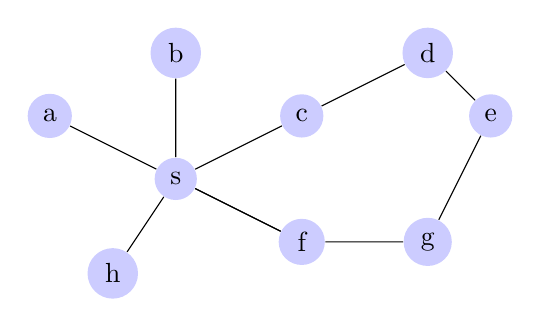
\begin{tikzpicture}
[scale=.8,auto=left,every node/.style={circle,fill=blue!20}]
\node (s) at (5,5) {s};
\node (a) at (3,6) {a};
\node (b) at (5,7) {b};
\node (c) at (7,6) {c};
\node (d) at (9,7) {d};
\node (e) at (10,6) {e};
\node (f) at (7,4) {f};
\node (g) at (9,4) {g};
\node (h) at (4,3.5) {h};
\foreach \from/\to in {s/a,s/b,s/c,s/f,s/h,c/d,d/e,e/g,g/f,f/s}
	\draw (\from) -- (\to);
\end{tikzpicture} 
\\\\
Assuming that all edges have the same length, and for $k=5$, the initial claim would give us a 5-collection path of vertices: {s,a,s,b,s,c,s,f,s,h,s}. This path has length 10. 
\\\\
However, the following path: {s,c,d,e,g,f,s}, has a length of 6. It is obvious that the second path is shorter even though it has vertices that are further away from s. 

\problempart 

In order to make sure that all the chickens will end up at the fenced field s, what we have to do is visit all the edges (but s) in a reverse BFS order. So basically what we need to do is a topological BFS sort of the nodes and visit them in that order.
\\\\
We would begin by running a Breadth-First search on the graph, starting with node s and recursing until we visit all the nodes. Once we have the order that the BFS visited the nodes, we can visit the nodes in the opposite order. Starting with the outer (more distant) level, we work ourselves in, level by level.
\\\\
Since this is exactly the opposite order of BFS, this will take us O(V+E) time, exactly as it would take for a Breadth-First search.


\problempart 
We could easily do that in two ways. The first way would be to just visit node s after we visited all other nodes and we forced chickens to go there. The other way would be to visit the nodes in regular BFS order. In both cases the chicken wants to leave because you are there but also it has nowhere to go because you have either visited the fields it can go to, or it is uphill.

\end{problemparts}

\section*{Part B}

\problem
\begin{problemparts}
\problempart \emph{On alg.csail.mit.edu}
\problempart \emph{On alg.csail.mit.edu}
\problempart 
The idea behind this algorithm is very similar to that of the EXACTSEARCH algorithm.
The difference however, is that we need to check if the sliding window hashes to the same value as any of the possible strings that result from replacing any letter of the pattern with an unknown character '?'. 
\\\\
We begin by adding the unknown character "?" into our alphabet and assigning it to an arbitrary value and making a hash table with all the possible strings we want to search for. In order to create H efficiently, we want to calculate the hash of each of the strings recursively. That is for every character in the pattern, we loop through every character after it and change it to "?", then we calculate the hash value for the string, and insert it in the hash table. We perform this for all characters in the pattern. Since every loop execution takes O(1) time and there are $O(2^k)$ loops (since there are this many strings), this would take $O(2^k)$ time. 
\\\\
Once we have our hash table ready, we can perform the EXACTSEARCH algorithm with some minor changes. Namely, instead of comparing the value of the rolling hash with the value of the hashing of the pattern, we just check if the value of the rolling hash is in the hash table we created (of the hash values of all the possible strings that result from changing any character to "?"). This check takes O(1) time.
\\\\
Since we need $O(2^k)$ time to create this hash table and we need to do $O(n)$ checks of time $O(1)$, 
our total runtime will be:
\begin{align*}
T(n)=O(2^k)+O(n*1)\Longleftrightarrow T(n)=O(2^k+n)
\end{align*}

\end{problemparts}

\end{problems}

\end{document}

